\chapter{Project Overview}
In order to present a practical solution and application of the discussed modular development approach to development of complex software systems, a project have been developed to support the theory and show the way it can be achieved. Some aspects of the implementation have been left out for the reason of being trivial and basic when it comes to android development, areas such as layout design, environment configuration, values and drawable settings, this aspects are unique from developer to developer and can be set as pleased. Though some important pointers will be stated where deemed.

This project is a surveillance application which i named "Eye Droid". The idea behind it is to develop an Android application that will make use of an android device camera to monitor a particular surrounding, notifying the user in real time, whenever a face is detected. This is a great idea considering there are lots of android devices out there ranging from mobile phones, native cameras, tablets and other embedded devices.

The project will cover the structure of the system, the system models showing different perspectives of the system including use case diagram,  class diagram and show the screen shot of each activity. Also the implementation of the individual module that constitutes this software system will be discussed in detail along side the code snippets. 

\section{System Structure}
The architectural representation of this system shows the high-level structures of the software system. The structure of how the modules fit into the system is shown by the architectural diagram of the system followed by the brief description of each module.

\begin{figure}[ht!]
\centering
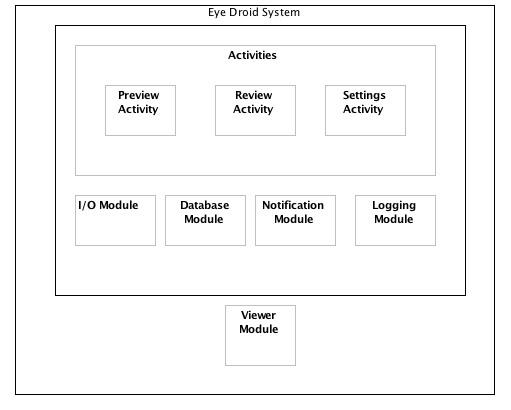
\includegraphics[width=140mm]{eye_arch.png}
\caption{Eye Droid System Architecture}
\label{overflow}
\end{figure}    

Modules present in this system as shown in listing 4.1 are the {\it I/O module, database module, notification module, logging module and viewer module}. The modules a structured in terms of packages (as the Java programming language provides us the means to modularize using this feature) except for the viewer module which is an application level module, and its installed separately in the system then called through the use of {\bf intents}. Apart from the modules implementation of the application, activities are also discussed. 

\begin{itemize}
\item {\bf I/O module}, this module contains a set of methods defined to handle different types of input and output operations. This module is used by the system Activities and also by some modules as they require some I/O operations.

\item{\bf Database module}, this module is responsible for the SQLite database connection, reads and writes. It is also used by the notification module to log some certain events that happened during the camera preview.

\item{\bf Notification module}, this modules deals with the EMAIL connection, sending of messages and attachments when it is called. This module is used by the Preview activity when notifying the user when a face is detected and also by the review activity when uploading the log file generated from the database.
 
\item{\bf Logging module}, this module is an android service, it is automatically started when the preview activity is started and it runs in the background listening to some certain events and logging them into the SQLite database using the database module.

\item{\bf Viewer module}, this module is an application level module developed using the Kivy framework, it is a simple image viewer module that displays images of faces detected and provide small features like enlarging, shrinking and rotation. It is called by the Main activity through intents.
\end{itemize}
The application also contains user settings informations, information such as email, password, phone number e.t.c This information are stored in the user preferences, which is a file that exist in the system and can be read or written into very easily.

\section{Activities}
Activities are the presentation layer of an Android application, an application consist of one or more activities and an activity can pass data or control to another activity by the use of the interprocess communication protocol called {\bf intents}. Each activity consist of a single visual user interface (that is what the user sees with the buttons and images e.t.c) designed using XML and accompanied by a java class which contains the code responsible for handling the various types of widgets in the GUI. In this thesis i will not discuss the graphical representation of an activity as it is basics and anyone can get a hang of it, however i will discuss the back-end code responsible for handling this views.

Each activity has a structure and a set of events that can be implemented to control the lifecycle of the activity. Each event is a method that is called depending on what phase the activity is in the lifecycle.

\begin{figure}[ht!]
\centering
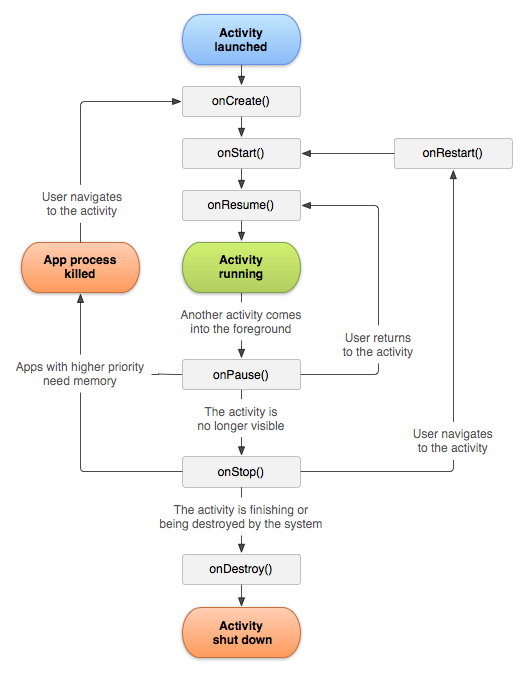
\includegraphics[width=110mm]{activity_lifecycle.png}
\caption{Android Activity lifecycle}
\label{overflow}
\end{figure}

\begin{itemize}
\item{\bf onCreate()} This is called when the activity is started, and to perform a one-time initialization of objects instances leading to the launch of the individual interface. It contains a parameter that has information gotten from the {\it onSaveInstanceState()} method which is the previous state of the activity and can be null if there was no previously saved state.
\item{\bf onStart()} This is called after the {\it onCreate()} method have complete initialization and content is ready to be shown to the user.
\item{\bf onResume()} This is called when the activity is to be brought to the foreground and ready to continue from where it was left off.
\item{\bf onRestart()} This event is triggered after an activity have been stopped (not paused) and started again. Which in other words the activity is redisplayed to the user.
\item{\bf onPause()} this is triggered when another activity is brought to the foreground, either by the user when navigating to another activity of because another application with higher priority needs memory.
\item{\bf onStop()} This is called when the activity is no longer visible. If there is need for memory, this event can also be triggered by the OS.
\item{\bf onDestroy()} This is called just before the activity is destroyed, either by the user finishing the activity or by the system when it needs memory.
\end{itemize}

The following are the list of activities present in the {\bf Eye Droid} project:
\begin{itemize}
\item{\bf Main activity}, as the name implies, this is the first screen a user will see after the splash screen. It contains various image buttons that leads to different activities. The preview button, review button, settings button and viewer button.
\item{\bf Preview Activity}, this is the activity that captures the camera preview, and detects faces, it displays the preview alongside the number of face label and the capture button.
\item{\bf Review Activity}, simply displays the log content to the user, and provides option to either wipe clean the log or upload the log.
\item{\bf Settings Activity}, this activity provides an interface for the user to set email, password, phone number e.t.c and save to the user preferences. 
\end{itemize} 

\section{Intent}
{\bf Intent} is an abstract description of an operation to be performed, it allows application components to request functionalities from other android components. {\it startActivity} can be used to launch an activity and {\it startService(Intent)} to start and communicate with a background service.

An intent structure contains 6 parts:
\begin{itemize}
\item {\bf action}, the action to be performed e.g "ACTION\_VIEW", "ACTION\_DIAL"
\item {\bf data}, the data to be acted upon
\item {\bf category}, information on the action to be executed
\item {\bf type}, explicitly specifies the type of intent data
\item {\bf component}, explicitly specifies the name of the component to be used by the intent
\item {\bf extras}, a Bundle which contains additional information for the component.
\end{itemize}
